% The MIT License (MIT)
%
% Copyright (c) 2020 Yegor Bugayenko
%
% Permission is hereby granted, free of charge, to any person obtaining a copy
% of this software and associated documentation files (the "Software"), to deal
% in the Software without restriction, including without limitation the rights
% to use, copy, modify, merge, publish, distribute, sublicense, and/or sell
% copies of the Software, and to permit persons to whom the Software is
% furnished to do so, subject to the following conditions:
%
% The above copyright notice and this permission notice shall be included
% in all copies or substantial portions of the Software.
%
% THE SOFTWARE IS PROVIDED "AS IS", WITHOUT WARRANTY OF ANY KIND, EXPRESS OR
% IMPLIED, INCLUDING BUT NOT LIMITED TO THE WARRANTIES OF MERCHANTABILITY,
% FITNESS FOR A PARTICULAR PURPOSE AND NON-INFRINGEMENT. IN NO EVENT SHALL THE
% AUTHORS OR COPYRIGHT HOLDERS BE LIABLE FOR ANY CLAIM, DAMAGES OR OTHER
% LIABILITY, WHETHER IN AN ACTION OF CONTRACT, TORT OR OTHERWISE, ARISING FROM,
% OUT OF OR IN CONNECTION WITH THE SOFTWARE OR THE USE OR OTHER DEALINGS IN THE
% SOFTWARE.

\documentclass[anonymous,sigconf,10pt,nonacm=true]{acmart}
\title{...}
\author{Yegor Bugayenko}{}{}
\email{yegor.bugayenko@huawei.com}
\affiliation{%
  \institution{Huawei Technologies Co., Ltd.}
  \city{Moscow, Russia}
}
\ccsdesc[100]{Object-Oriented Programming}
\keywords{OOP, Naming, Code Quality}

\usepackage[utf8]{inputenc}
\usepackage{textcomp}
\usepackage[inline]{enumitem}
\usepackage{amsmath}
\usepackage{graphicx}
\usepackage{pgfplots}
\usepackage{verbatimbox}
\usepackage{interval}
\usepackage{hyperref}
\usepackage{minted}
  \setminted{fontsize=\footnotesize}
  \setminted{breaklines}
  \usemintedstyle{bw}
\newcommand{\code}[1]{\texttt{#1}}
\newenvironment{nicetable}
  {\setlength{\parindent}{0em}\medskip\small}
  {\medskip}
\begin{document}
\begin{abstract}
...
\end{abstract}
\maketitle

\section{Introduction}

...

The paper is organized as follows.
Section~\ref{sec:background} defines various terms used in the paper.
Section~\ref{sec:related} covers related work ...
Section~\ref{sec:method} covers the method of research.
Section~\ref{sec:results} covers our empirical case study.
Section~\ref{sec:discussion} covers limitations of both the metric and the study.
Finally, we summarize our study in Section~\ref{sec:conclusion}.

\section{Background}
\label{sec:background}

...

\section{Related Work}
\label{sec:related}

...

\section{Metric}
\label{sec:method}

...

\section{Empirical Results}
\label{sec:results}

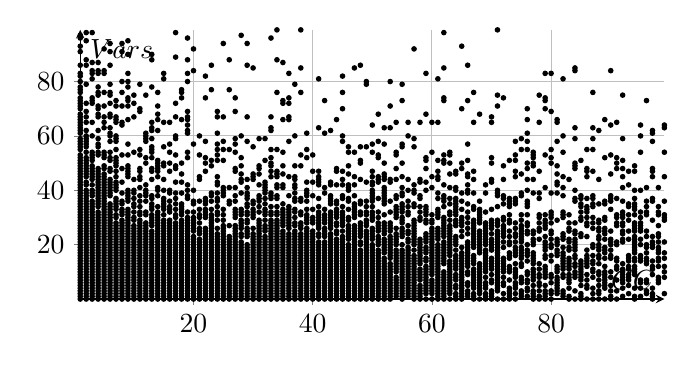
\begin{tikzpicture}
\begin{axis}[width=9cm,height=5cm,
axis lines=middle, xlabel={$CC$}, ylabel={$Vars$},
xmin=1, xmax=99,
ymin=0, ymax=99,
extra tick style={major grid style=black},grid=major]
\addplot [mark=*, only marks, mark size=0.8pt] coordinates {
(1,0)
(5,0)
(2,0)
(7,0)
(3,0)
(6,1)
(1,1)
(5,11)
(13,2)
(4,1)
(5,2)
(367,52)
(18,5)
(16,13)
(42,19)
(4,0)
(52,27)
(25,4)
(52,18)
(6,0)
(13,1)
(44,20)
(23,10)
(35,46)
(10,3)
(12,2)
(48,12)
(17,4)
(14,6)
(38,2)
(15,3)
(10,10)
(14,3)
(23,9)
(22,8)
(16,7)
(9,2)
(11,8)
(12,0)
(49,9)
(39,13)
(10,0)
(9,1)
(16,3)
(8,1)
(9,6)
(24,6)
(86,14)
(14,8)
(74,10)
(21,6)
(53,9)
(20,4)
(30,5)
(22,0)
(31,1)
(1,2)
(108,22)
(18,3)
(7,1)
(24,2)
(27,13)
(6,2)
(2,1)
(2,3)
(8,3)
(28,5)
(2,2)
(3,1)
(15,4)
(55,26)
(8,0)
(87,37)
(90,37)
(4,6)
(3,12)
(3,2)
(11,3)
(4,4)
(11,0)
(34,21)
(79,27)
(74,23)
(24,11)
(42,10)
(23,14)
(2,4)
(6,4)
(49,28)
(26,27)
(6,5)
(11,14)
(17,1)
(11,4)
(17,5)
(9,3)
(9,0)
(4,2)
(37,5)
(41,4)
(14,5)
(17,10)
(15,0)
(17,6)
(104,23)
(13,8)
(55,7)
(12,16)
(26,3)
(101,47)
(30,16)
(12,7)
(46,15)
(38,18)
(54,15)
(22,7)
(27,14)
(16,4)
(8,2)
(12,1)
(7,3)
(7,2)
(5,8)
(7,4)
(9,5)
(5,1)
(39,25)
(37,18)
(70,11)
(15,5)
(26,10)
(21,2)
(26,6)
(44,16)
(9,4)
(17,12)
(6,9)
(11,10)
(10,8)
(15,2)
(16,12)
(44,5)
(3,3)
(5,6)
(40,1)
(1,3)
(2,8)
(1,11)
(11,7)
(5,5)
(8,22)
(18,19)
(7,17)
(5,3)
(19,7)
(10,9)
(10,1)
(1,32)
(4,16)
(7,9)
(1,18)
(1,6)
(28,20)
(31,4)
(13,3)
(12,6)
(18,1)
(1,10)
(6,6)
(12,15)
(76,70)
(2,10)
(46,3)
(21,5)
(38,14)
(12,3)
(1,9)
(1,4)
(10,7)
(2,9)
(1,7)
(1,5)
(11,1)
(41,6)
(8,4)
(10,5)
(14,22)
(4,17)
(2,13)
(1,8)
(3,4)
(10,12)
(1,38)
(2,19)
(19,0)
(23,3)
(13,0)
(1,15)
(6,28)
(2,12)
(6,11)
(1,14)
(10,2)
(89,24)
(16,20)
(42,5)
(19,4)
(8,6)
(7,11)
(20,11)
(13,5)
(4,7)
(12,4)
(2,7)
(10,6)
(10,4)
(39,9)
(22,1)
(17,2)
(26,5)
(3,9)
(4,8)
(5,4)
(30,10)
(30,1)
(27,6)
(21,0)
(20,2)
(87,20)
(19,3)
(11,2)
(7,6)
(8,15)
(14,2)
(27,8)
(3,5)
(22,5)
(22,20)
(17,0)
(19,8)
(4,3)
(38,5)
(2,18)
(3,10)
(18,9)
(91,0)
(113,9)
(14,0)
(34,6)
(57,35)
(52,4)
(25,8)
(155,17)
(20,12)
(16,6)
(189,16)
(15,9)
(9,8)
(76,20)
(2,6)
(62,6)
(40,18)
(25,9)
(13,7)
(6,7)
(3,7)
(4,20)
(3,11)
(11,32)
(6,63)
(3,6)
(25,13)
(6,3)
(29,12)
(7,10)
(21,9)
(7,25)
(23,2)
(15,1)
(14,1)
(4,5)
(60,9)
(1,21)
(29,15)
(119,4)
(198,19)
(68,2)
(30,3)
(61,1)
(30,6)
(152,8)
(49,2)
(24,0)
(51,3)
(15,7)
(21,1)
(118,1)
(29,2)
(180,1)
(59,0)
(21,11)
(18,13)
(29,6)
(20,1)
(6,10)
(27,2)
(9,13)
(38,1)
(17,16)
(24,3)
(43,15)
(16,1)
(26,1)
(1,13)
(1,19)
(9,9)
(19,23)
(50,1)
(50,25)
(6,12)
(34,37)
(2,5)
(2,36)
(8,7)
(14,4)
(18,50)
(24,5)
(29,1)
(20,0)
(30,2)
(63,8)
(46,6)
(22,16)
(20,6)
(15,23)
(35,3)
(6,61)
(15,65)
(1,12)
(16,5)
(3,16)
(2,11)
(11,11)
(42,11)
(1,17)
(5,17)
(29,140)
(3,18)
(10,19)
(5,9)
(15,17)
(22,9)
(22,10)
(31,24)
(14,9)
(21,33)
(7,5)
(24,10)
(6,8)
(12,11)
(23,7)
(27,9)
(3,14)
(95,64)
(66,13)
(50,2)
(37,1)
(18,0)
(7,7)
(109,55)
(30,14)
(15,13)
(27,4)
(18,6)
(12,8)
(33,21)
(12,19)
(17,18)
(31,0)
(96,13)
(34,55)
(30,24)
(153,18)
(22,2)
(16,11)
(7,16)
(11,38)
(7,15)
(11,5)
(38,26)
(25,11)
(16,0)
(4,23)
(3,8)
(7,20)
(13,9)
(12,5)
(3,25)
(19,67)
(27,47)
(1,20)
(4,15)
(3,24)
(57,13)
(8,9)
(45,4)
(57,16)
(23,15)
(14,11)
(14,62)
(17,14)
(1,16)
(32,10)
(17,3)
(21,21)
(43,27)
(119,214)
(22,15)
(27,15)
(43,42)
(23,13)
(16,2)
(9,48)
(2,25)
(21,12)
(17,9)
(41,14)
(45,0)
(38,3)
(19,1)
(22,12)
(46,4)
(5,18)
(46,12)
(11,13)
(24,51)
(5,14)
(60,28)
(33,22)
(23,6)
(9,7)
(74,45)
(25,0)
(39,4)
(50,18)
(21,16)
(4,34)
(5,34)
(15,6)
(2,30)
(14,30)
(1,51)
(6,14)
(26,14)
(66,86)
(4,12)
(1,42)
(42,16)
(1,22)
(11,6)
(24,23)
(46,13)
(13,12)
(88,15)
(48,2)
(28,17)
(22,3)
(41,18)
(17,7)
(13,4)
(59,29)
(52,22)
(27,3)
(19,10)
(35,7)
(72,11)
(31,15)
(25,2)
(35,4)
(37,7)
(23,12)
(26,4)
(8,5)
(16,9)
(31,7)
(1,49)
(4,31)
(4,19)
(1,59)
(8,23)
(31,2)
(39,7)
(42,7)
(35,6)
(18,8)
(44,0)
(85,10)
(29,4)
(30,4)
(19,2)
(25,5)
(36,3)
(18,2)
(24,4)
(23,1)
(24,8)
(40,4)
(28,3)
(17,8)
(27,0)
(40,3)
(29,3)
(25,14)
(38,7)
(57,26)
(115,79)
(43,14)
(40,14)
(45,20)
(48,28)
(106,19)
(36,15)
(23,0)
(28,0)
(26,0)
(43,16)
(21,13)
(5,13)
(2,14)
(37,24)
(4,10)
(42,9)
(47,1)
(18,4)
(34,5)
(61,14)
(47,5)
(2,302)
(8,25)
(27,1)
(51,5)
(55,5)
(34,1)
(137,21)
(86,5)
(32,8)
(68,3)
(52,3)
(39,26)
(16,19)
(18,12)
(13,6)
(54,21)
(87,16)
(27,19)
(23,18)
(81,16)
(75,27)
(23,5)
(95,27)
(220,27)
(7,8)
(20,3)
(33,16)
(29,16)
(3,20)
(5,30)
(2,16)
(1,72)
(1,33)
(5,7)
(19,6)
(45,7)
(41,5)
(47,6)
(31,8)
(28,14)
(37,14)
(14,7)
(33,9)
(18,10)
(20,8)
(32,6)
(24,1)
(20,7)
(117,26)
(35,10)
(63,14)
(3,19)
(51,10)
(61,22)
(51,11)
(58,7)
(65,12)
(55,12)
(48,18)
(71,18)
(93,31)
(41,0)
(38,9)
(34,7)
(3,22)
(1,25)
(1,30)
(3,36)
(12,23)
(7,18)
(5,49)
(21,7)
(26,12)
(25,6)
(40,23)
(27,7)
(42,12)
(14,24)
(12,14)
(16,8)
(23,28)
(10,26)
(4,22)
(5,44)
(1,39)
(2,15)
(35,13)
(24,7)
(60,23)
(36,9)
(22,6)
(35,8)
(22,4)
(55,8)
(56,3)
(28,6)
(32,5)
(21,20)
(48,11)
(58,13)
(28,2)
(21,8)
(58,10)
(44,9)
(59,12)
(68,31)
(76,10)
(28,7)
(44,6)
(33,3)
(43,0)
(67,20)
(41,2)
(93,5)
(2,32)
(28,52)
(4,37)
(72,29)
(76,61)
(183,2)
(41,29)
(115,7)
(158,27)
(125,23)
(57,28)
(50,19)
(42,13)
(52,38)
(61,20)
(42,18)
(12,13)
(4,18)
(5,12)
(1,74)
(1,28)
(33,8)
(36,8)
(90,15)
(7,12)
(62,17)
(83,13)
(16,15)
(11,20)
(10,22)
(45,13)
(30,19)
(55,9)
(39,1)
(108,26)
(60,19)
(28,15)
(58,17)
(33,0)
(29,9)
(49,10)
(75,8)
(1,23)
(1,40)
(16,27)
(5,53)
(27,10)
(1,36)
(3,53)
(2,21)
(3,31)
(1,27)
(5,10)
(9,32)
(33,14)
(20,9)
(45,12)
(84,15)
(156,38)
(63,7)
(32,7)
(64,7)
(84,19)
(36,7)
(55,3)
(35,0)
(12,32)
(53,71)
(34,8)
(37,12)
(57,20)
(20,10)
(64,11)
(53,10)
(19,5)
(47,10)
(48,1)
(27,12)
(36,4)
(36,11)
(51,2)
(83,6)
(28,8)
(3,42)
(19,11)
(20,19)
(66,73)
(7,19)
(18,11)
(37,8)
(51,7)
(21,3)
(48,7)
(48,4)
(61,3)
(1,91)
(1,34)
(1,29)
(12,31)
(4,108)
(18,7)
(34,10)
(25,20)
(38,27)
(69,15)
(41,32)
(4,9)
(21,4)
(2,31)
(5,16)
(2,37)
(25,7)
(3,13)
(5,42)
(9,19)
(3,21)
(2,20)
(5,132)
(2,34)
(2,29)
(5,48)
(8,28)
(20,27)
(5,23)
(35,5)
(32,0)
(86,18)
(46,7)
(45,19)
(31,16)
(47,18)
(55,16)
(60,10)
(38,21)
(48,10)
(49,13)
(38,32)
(73,21)
(19,20)
(44,12)
(62,16)
(47,11)
(25,10)
(64,15)
(28,4)
(34,4)
(50,9)
(94,22)
(31,9)
(50,6)
(6,75)
(2,45)
(1,45)
(5,22)
(10,40)
(1,50)
(1,24)
(1,97)
(4,41)
(1,73)
(40,5)
(47,3)
(41,8)
(34,14)
(64,23)
(36,20)
(54,65)
(40,43)
(58,20)
(69,22)
(23,21)
(23,8)
(19,9)
(33,10)
(43,4)
(58,11)
(10,11)
(39,15)
(52,15)
(17,11)
(19,15)
(55,34)
(7,23)
(42,73)
(128,58)
(47,13)
(94,28)
(26,2)
(137,33)
(30,12)
(49,5)
(53,32)
(39,16)
(94,25)
(59,14)
(13,10)
(29,10)
(50,22)
(162,77)
(69,10)
(60,18)
(49,18)
(11,70)
(14,40)
(6,67)
(8,14)
(9,23)
(3,29)
(1,35)
(16,17)
(4,26)
(4,11)
(17,13)
(1,57)
(51,23)
(324,58)
(84,22)
(53,1)
(28,29)
(130,25)
(115,53)
(319,76)
(26,8)
(79,10)
(102,18)
(32,3)
(121,22)
(76,9)
(90,22)
(11,9)
(33,13)
(94,11)
(175,44)
(59,3)
(29,5)
(51,4)
(128,16)
(147,26)
(151,33)
(75,24)
(123,32)
(58,9)
(45,16)
(50,7)
(29,7)
(24,17)
(102,9)
(89,7)
(10,17)
(34,2)
(40,10)
(31,5)
(36,19)
(41,45)
(6,13)
(4,62)
(3,26)
(87,26)
(31,3)
(16,10)
(29,8)
(50,4)
(60,3)
(90,5)
(36,0)
(31,17)
(23,4)
(38,10)
(51,12)
(33,4)
(3,49)
(40,11)
(39,6)
(63,6)
(3,15)
(4,25)
(4,13)
(2,17)
(43,9)
(31,14)
(12,18)
(13,20)
(80,16)
(25,3)
(135,5)
(56,9)
(47,12)
(33,7)
(21,10)
(31,11)
(55,0)
(27,18)
(56,31)
(28,43)
(18,16)
(12,17)
(7,14)
(6,23)
(1,26)
(61,45)
(15,20)
(13,54)
(9,53)
(33,5)
(40,2)
(48,14)
(77,0)
(43,8)
(41,3)
(65,5)
(86,7)
(96,7)
(60,16)
(42,4)
(63,13)
(32,2)
(33,18)
(27,17)
(9,37)
(23,11)
(50,10)
(92,25)
(61,15)
(7,22)
(13,13)
(12,10)
(26,17)
(10,25)
(4,14)
(51,16)
(12,28)
(23,23)
(16,57)
(138,75)
(33,6)
(20,18)
(52,0)
(7,13)
(11,23)
(15,10)
(14,13)
(37,49)
(35,15)
(44,2)
(30,7)
(21,25)
(75,55)
(25,19)
(15,16)
(6,17)
(44,1)
(51,17)
(19,37)
(17,60)
(49,79)
(5,27)
(24,45)
(5,33)
(5,29)
(5,63)
(41,47)
(23,31)
(17,30)
(19,69)
(31,32)
(7,60)
(22,82)
(35,23)
(9,21)
(27,101)
(35,87)
(14,45)
(142,68)
(19,83)
(8,18)
(46,54)
(37,44)
(22,112)
(34,3)
(8,10)
(3,81)
(69,23)
(6,33)
(18,46)
(25,67)
(10,16)
(4,38)
(2,22)
(6,48)
(9,39)
(8,11)
(28,97)
(32,32)
(47,33)
(10,39)
(62,85)
(53,22)
(55,56)
(32,43)
(47,54)
(24,32)
(67,106)
(51,58)
(18,27)
(38,53)
(33,49)
(70,26)
(22,18)
(11,26)
(36,45)
(9,33)
(16,24)
(11,12)
(11,25)
(281,176)
(19,42)
(59,8)
(10,30)
(76,55)
(107,117)
(9,14)
(82,19)
(80,8)
(216,68)
(143,57)
(139,66)
(83,21)
(115,156)
(45,1)
(32,42)
(6,100)
(41,10)
(43,10)
(13,17)
(7,21)
(67,65)
(13,23)
(32,125)
(15,34)
(27,20)
(24,21)
(56,8)
(48,13)
(54,10)
(28,16)
(14,12)
(31,34)
(67,15)
(125,21)
(8,12)
(25,17)
(36,24)
(26,7)
(62,2)
(28,9)
(70,33)
(7,105)
(10,21)
(15,11)
(13,34)
(2,27)
(17,26)
(17,31)
(27,32)
(24,24)
(44,13)
(6,20)
(23,86)
(7,43)
(9,28)
(11,41)
(131,46)
(20,16)
(79,70)
(17,35)
(78,5)
(86,30)
(66,1)
(38,15)
(76,3)
(54,18)
(76,50)
(84,49)
(50,16)
(125,51)
(44,35)
(122,68)
(63,11)
(18,31)
(33,52)
(6,16)
(64,37)
(39,33)
(48,32)
(134,38)
(49,27)
(9,10)
(33,19)
(43,35)
(62,98)
(15,18)
(55,73)
(77,50)
(19,28)
(21,22)
(12,27)
(60,13)
(47,24)
(98,32)
(75,18)
(158,32)
(40,7)
(22,14)
(3,17)
(62,7)
(48,3)
(28,1)
(34,0)
(43,3)
(25,1)
(7,27)
(36,67)
(25,33)
(38,0)
(60,24)
(71,10)
(69,39)
(20,5)
(91,28)
(74,11)
(53,3)
(30,8)
(101,17)
(66,57)
(60,17)
(42,3)
(29,94)
(35,21)
(8,17)
(39,18)
(75,19)
(76,40)
(39,0)
(76,36)
(301,109)
(73,1)
(133,4)
(8,8)
(68,5)
(36,6)
(52,1)
(46,14)
(7,30)
(135,36)
(102,5)
(122,55)
(373,192)
(119,28)
(187,46)
(97,1)
(10,29)
(8,29)
(13,25)
(13,56)
(5,20)
(94,129)
(2,52)
(4,45)
(4,78)
(50,142)
(13,44)
(9,11)
(18,76)
(20,17)
(23,19)
(44,42)
(30,56)
(32,29)
(16,22)
(12,59)
(56,60)
(57,156)
(14,16)
(3,74)
(47,20)
(52,6)
(12,21)
(64,0)
(107,296)
(53,194)
(153,111)
(71,7)
(71,34)
(75,148)
(4,39)
(211,113)
(127,114)
(143,106)
(5,21)
(25,29)
(78,75)
(40,0)
(31,13)
(172,46)
(93,42)
(14,10)
(19,54)
(59,43)
(9,17)
(39,8)
(51,0)
(65,3)
(70,0)
(635,101)
(788,98)
(21,18)
(13,21)
(37,36)
(15,8)
(110,10)
(65,7)
(131,1)
(29,0)
(105,0)
(409,25)
(68,4)
(93,12)
(61,13)
(79,11)
(63,23)
(66,16)
(48,0)
(50,13)
(37,10)
(146,54)
(75,7)
(194,79)
(21,14)
(259,0)
(257,75)
(76,25)
(83,14)
(57,7)
(69,5)
(92,13)
(117,46)
(146,63)
(66,3)
(139,59)
(23,29)
(200,83)
(56,21)
(63,53)
(38,8)
(39,17)
(62,74)
(31,6)
(51,22)
(28,33)
(18,77)
(14,48)
(45,6)
(81,5)
(62,9)
(88,9)
(52,2)
(31,21)
(104,33)
(579,45)
(132,15)
(128,24)
(106,24)
(78,9)
(47,4)
(92,7)
(25,12)
(43,20)
(15,12)
(51,13)
(75,6)
(37,6)
(41,23)
(249,7)
(102,32)
(36,14)
(71,11)
(70,13)
(73,36)
(88,26)
(30,0)
(94,0)
(61,0)
(115,0)
(78,0)
(37,0)
(35,2)
(107,0)
(6,29)
(56,22)
(13,11)
(43,7)
(49,4)
(31,10)
(60,7)
(33,15)
(29,13)
(22,11)
(75,15)
(19,12)
(82,1)
(74,6)
(40,13)
(47,16)
(102,0)
(49,34)
(45,2)
(56,18)
(127,19)
(46,0)
(54,2)
(44,24)
(30,20)
(24,15)
(16,40)
(13,16)
(110,103)
(91,7)
(34,9)
(60,0)
(30,17)
(208,62)
(78,31)
(51,14)
(77,25)
(378,102)
(93,35)
(63,50)
(67,8)
(55,14)
(38,16)
(35,28)
(52,5)
(58,16)
(52,44)
(42,0)
(43,1)
(134,15)
(24,14)
(45,25)
(124,33)
(56,2)
(105,4)
(203,0)
(65,10)
(20,13)
(30,23)
(71,25)
(25,15)
(77,24)
(67,44)
(32,41)
(59,4)
(191,26)
(22,13)
(30,30)
(15,19)
(30,15)
(20,57)
(53,12)
(86,23)
(214,42)
(37,2)
(35,14)
(127,9)
(63,17)
(32,33)
(82,11)
(77,9)
(74,21)
(91,11)
(52,8)
(246,12)
(136,27)
(64,14)
(29,23)
(74,252)
(260,349)
(44,32)
(1,64)
(4,27)
(6,15)
(3,173)
(14,66)
(32,4)
(11,18)
(3,45)
(9,15)
(2,54)
(18,66)
(8,13)
(9,29)
(25,21)
(86,37)
(1,37)
(9,16)
(12,22)
(1,65)
(19,22)
(9,26)
(11,31)
(35,73)
(41,21)
(1,48)
(13,62)
(9,95)
(26,41)
(9,18)
(8,65)
(29,108)
(4,53)
(15,153)
(18,35)
(20,28)
(7,65)
(6,30)
(4,36)
(8,19)
(6,19)
(4,67)
(8,80)
(28,143)
(17,15)
(12,61)
(7,40)
(29,26)
(13,112)
(13,31)
(10,183)
(16,39)
(3,44)
(13,63)
(20,84)
(11,148)
(4,29)
(4,68)
(4,56)
(6,21)
(14,138)
(2,48)
(24,36)
(44,146)
(8,71)
(1,107)
(9,90)
(7,51)
(2,88)
(13,35)
(10,27)
(18,34)
(55,10)
(5,24)
(7,52)
(7,31)
(30,44)
(4,84)
(55,38)
(20,14)
(2,38)
(51,32)
(71,40)
(40,20)
(39,19)
(94,47)
(14,14)
(32,17)
(18,21)
(70,21)
(69,6)
(37,21)
(76,18)
(37,17)
(98,24)
(43,11)
(34,17)
(60,21)
(42,20)
(26,15)
(96,2)
(32,39)
(75,39)
(11,17)
(107,59)
(63,32)
(46,27)
(34,12)
(53,28)
(93,34)
(129,41)
(69,11)
(46,9)
(39,28)
(74,18)
(141,49)
(31,29)
(65,27)
(111,79)
(33,11)
(79,53)
(52,40)
(16,14)
(26,11)
(31,27)
(45,34)
(29,11)
(29,18)
(63,16)
(25,25)
(41,27)
(15,14)
(46,37)
(51,37)
(38,24)
(60,45)
(68,18)
(93,25)
(32,14)
(40,22)
(19,14)
(140,63)
(32,16)
(44,10)
(80,20)
(60,26)
(38,19)
(28,19)
(117,28)
(26,22)
(36,1)
(18,25)
(27,26)
(13,18)
(42,41)
(10,15)
(113,35)
(99,21)
(73,17)
(47,8)
(36,10)
(79,20)
(43,23)
(61,18)
(10,13)
(43,5)
(30,13)
(39,20)
(18,14)
(46,2)
(60,31)
(41,1)
(36,23)
(46,18)
(52,21)
(47,38)
(76,28)
(56,40)
(20,21)
(14,25)
(45,60)
(12,24)
(63,22)
(134,112)
(38,12)
(150,72)
(38,6)
(17,17)
(31,28)
(71,38)
(67,24)
(53,44)
(163,99)
(102,36)
(80,55)
(66,5)
(37,9)
(52,28)
(62,25)
(181,113)
(85,5)
(135,30)
(24,43)
(32,20)
(30,18)
(27,16)
(63,41)
(22,22)
(12,38)
(26,23)
(22,17)
(76,66)
(8,26)
(24,37)
(9,12)
(54,20)
(7,28)
(46,30)
(100,21)
(154,3)
(255,14)
(73,4)
(77,10)
(63,4)
(131,5)
(78,6)
(130,41)
(66,40)
(35,19)
(13,14)
(36,2)
(85,14)
(47,7)
(89,8)
(71,19)
(5,15)
(6,24)
(31,18)
(23,17)
(24,18)
(17,19)
(190,23)
(83,4)
(39,14)
(93,22)
(86,27)
(139,10)
(117,17)
(123,1)
(42,8)
(72,19)
(111,41)
(381,173)
(39,5)
(16,25)
(82,3)
(50,0)
(834,0)
(117,0)
(74,0)
(44,33)
(74,26)
(64,27)
(46,16)
(151,65)
(283,40)
(212,3)
(55,15)
(24,13)
(166,17)
(86,13)
(123,4)
(55,24)
(35,30)
(49,20)
(29,20)
(38,4)
(55,1)
(53,2)
(12,20)
(42,31)
(116,121)
(35,12)
(61,39)
(95,7)
(460,2)
(458,0)
(97,0)
(146,0)
(55,4)
(49,19)
(39,3)
(83,11)
(67,6)
(32,1)
(35,11)
(57,18)
(63,20)
(68,20)
(26,19)
(59,32)
(47,2)
(86,33)
(32,11)
(149,15)
(14,23)
(7,24)
(13,28)
(6,39)
(28,11)
(10,23)
(17,24)
(45,32)
(120,40)
(62,14)
(4,30)
(60,5)
(52,11)
(111,47)
(46,36)
(47,25)
(55,11)
(70,44)
(59,11)
(56,16)
(318,32)
(62,23)
(51,18)
(111,17)
(107,10)
(39,2)
(105,14)
(37,13)
(54,16)
(44,17)
(155,4)
(146,2)
(136,2)
(57,12)
(198,47)
(157,59)
(19,21)
(5,28)
(7,247)
(2,40)
(18,32)
(66,259)
(9,36)
(2,67)
(67,21)
(35,17)
(49,15)
(56,5)
(82,22)
(122,49)
(34,20)
(24,9)
(1,31)
(95,22)
(8,27)
(14,34)
(57,8)
(14,26)
(9,45)
(59,15)
(38,28)
(66,17)
(5,35)
(62,8)
(107,3)
(69,26)
(45,5)
(41,16)
(122,26)
(35,9)
(22,50)
(8,35)
(7,26)
(4,48)
(5,212)
(28,31)
(5,43)
(9,116)
(14,27)
(28,10)
(26,18)
(58,14)
(32,15)
(218,55)
(34,15)
(26,20)
(3,54)
(10,54)
(24,61)
(42,29)
(54,33)
(36,26)
(37,4)
(32,13)
(53,13)
(47,15)
(36,16)
(121,79)
(45,9)
(55,25)
(54,53)
(48,23)
(55,23)
(37,22)
(7,45)
(12,60)
(29,14)
(10,14)
(12,9)
(14,19)
(46,19)
(32,9)
(29,24)
(73,10)
(28,46)
(42,2)
(68,6)
(56,14)
(19,64)
(5,26)
(11,27)
(27,5)
(101,6)
(29,35)
(21,24)
(27,11)
(8,16)
(90,142)
(33,96)
(6,34)
(77,49)
(37,45)
(14,49)
(8,32)
(3,27)
(22,32)
(37,42)
(17,59)
(10,126)
(27,57)
(60,65)
(15,49)
(15,50)
(15,21)
(32,27)
(18,29)
(25,51)
(22,58)
(66,30)
(4,32)
(17,20)
(3,84)
(4,54)
(23,27)
(24,53)
(6,31)
(12,36)
(24,120)
(29,58)
(13,37)
(8,24)
(38,17)
(45,58)
(7,49)
(30,26)
(50,29)
(19,80)
(84,28)
(13,15)
(12,50)
(23,16)
(9,47)
(3,23)
(17,49)
(62,1)
(34,13)
(46,49)
(7,41)
(34,99)
(1,76)
(5,32)
(47,26)
(1,47)
(16,65)
(11,15)
(6,26)
(38,85)
(11,24)
(65,70)
(46,24)
(8,31)
(6,25)
(42,26)
(43,30)
(12,42)
(13,19)
(2,33)
(23,77)
(30,115)
(25,26)
(52,46)
(84,59)
(21,31)
(31,42)
(18,28)
(27,74)
(23,20)
(12,12)
(11,22)
(18,15)
(79,23)
(14,20)
(48,15)
(23,25)
(50,15)
(32,25)
(61,51)
(17,89)
(33,26)
(40,28)
(37,32)
(52,36)
(46,42)
(6,47)
(17,39)
(22,47)
(8,20)
(23,49)
(81,66)
(29,86)
(48,51)
(33,50)
(27,31)
(14,47)
(12,58)
(24,57)
(19,61)
(2,35)
(12,39)
(19,16)
(71,99)
(10,34)
(76,151)
(14,17)
(26,16)
(45,76)
(50,119)
(15,25)
(40,47)
(27,25)
(54,128)
(47,85)
(24,39)
(22,24)
(5,19)
(4,136)
(4,59)
(59,48)
(2,42)
(9,24)
(6,22)
(6,44)
(6,18)
(15,31)
(4,42)
(34,27)
(27,54)
(41,44)
(19,52)
(35,16)
(59,31)
(50,36)
(24,20)
(4,47)
(16,18)
(22,31)
(24,34)
(21,30)
(25,24)
(132,10)
(118,51)
(21,15)
(26,13)
(35,18)
(130,48)
(68,17)
(44,7)
(65,29)
(40,6)
(34,18)
(58,30)
(139,88)
(34,46)
(60,6)
(51,30)
(150,62)
(141,46)
(104,70)
(36,33)
(21,17)
(14,15)
(37,19)
(45,42)
(49,23)
(31,12)
(61,16)
(46,11)
(183,59)
(82,16)
(64,32)
(105,55)
(81,43)
(90,18)
(65,13)
(43,12)
(80,19)
(53,4)
(93,14)
(61,11)
(44,15)
(69,20)
(108,27)
(38,13)
(40,9)
(28,12)
(51,53)
(54,23)
(191,17)
(110,13)
(72,30)
(45,14)
(114,23)
(42,6)
(53,8)
(104,39)
(130,35)
(113,31)
(106,31)
(62,27)
(72,24)
(95,15)
(30,11)
(178,14)
(54,6)
(58,18)
(43,2)
(98,19)
(96,20)
(46,5)
(183,5)
(61,33)
(85,51)
(36,27)
(68,7)
(45,28)
(19,18)
(28,24)
(53,26)
(26,9)
(20,15)
(72,2)
(71,8)
(68,68)
(109,78)
(51,44)
(59,22)
(51,25)
(62,21)
(48,5)
(78,22)
(163,54)
(37,16)
(67,28)
(52,7)
(67,16)
(43,19)
(146,23)
(88,20)
(77,21)
(44,8)
(37,3)
(44,11)
(91,15)
(52,13)
(36,12)
(109,31)
(69,24)
(62,15)
(115,13)
(91,20)
(56,4)
(34,16)
(31,22)
(36,83)
(107,22)
(115,31)
(131,24)
(39,22)
(72,44)
(37,27)
(14,21)
(2,24)
(25,22)
(81,8)
(6,72)
(71,15)
(52,35)
(16,21)
(375,0)
(33,24)
(464,65)
(116,10)
(238,137)
(270,3)
(70,1)
(235,15)
(2,23)
(36,66)
(30,137)
(6,27)
(22,21)
(15,40)
(74,36)
(32,51)
(10,20)
(45,22)
(11,19)
(10,18)
(83,0)
(41,11)
(37,15)
(34,41)
(38,20)
(8,232)
(3,46)
(1,93)
(51,143)
(1,41)
(23,164)
(22,158)
(4,208)
(6,91)
(2,43)
(41,63)
(8,64)
(26,35)
(11,21)
(5,38)
(3,40)
(48,9)
(54,1)
(47,0)
(55,6)
(80,30)
(83,26)
(1,53)
(13,48)
(6,52)
(4,28)
(12,75)
(40,29)
(15,37)
(17,28)
(1,43)
(30,154)
(35,32)
(6,38)
(3,39)
(21,36)
(7,42)
(65,39)
(44,47)
(72,13)
(45,10)
(59,9)
(43,18)
(57,23)
(307,26)
(98,12)
(87,2)
(48,6)
(117,4)
(144,11)
(134,9)
(70,7)
(33,2)
(64,31)
(13,24)
(82,2)
(104,0)
(51,1)
(14,18)
(2,26)
(31,37)
(16,23)
(9,30)
(11,47)
(3,33)
(9,66)
(16,28)
(70,43)
(17,98)
(54,3)
(83,9)
(130,16)
(76,1)
(75,3)
(30,36)
(16,54)
(10,24)
(23,108)
(53,153)
(34,45)
(6,40)
(17,72)
(6,42)
(103,103)
(9,57)
(5,37)
(19,118)
(13,55)
(5,25)
(4,24)
(32,151)
(60,54)
(36,13)
(46,25)
(76,48)
(48,26)
(57,34)
(66,14)
(104,43)
(87,28)
(58,44)
(94,26)
(45,15)
(18,18)
(91,50)
(28,60)
(16,47)
(41,81)
(8,33)
(7,66)
(13,38)
(14,41)
(4,21)
(14,115)
(5,45)
(1,52)
(6,139)
(9,73)
(13,59)
(2,51)
(2,69)
(5,67)
(20,23)
(23,39)
(16,33)
(6,79)
(5,71)
(3,51)
(61,32)
(30,9)
(46,40)
(48,20)
(35,31)
(40,17)
(17,23)
(72,23)
(57,21)
(46,20)
(187,64)
(50,31)
(72,38)
(22,35)
(9,78)
(13,90)
(79,31)
(9,20)
(12,26)
(21,192)
(28,28)
(255,53)
(15,15)
(16,29)
(7,34)
(34,76)
(50,45)
(15,56)
(80,3)
(317,31)
(105,2)
(129,56)
(49,0)
(49,6)
(9,22)
(20,22)
(69,28)
(7,36)
(19,17)
(55,50)
(45,18)
(33,28)
(3,72)
(11,209)
(50,20)
(9,31)
(58,1)
(15,44)
(37,39)
(131,16)
(206,32)
(168,29)
(99,36)
(134,21)
(1096,107)
(83,1)
(154,1)
(52,12)
(63,9)
(69,13)
(39,21)
(16,50)
(20,32)
(43,22)
(122,11)
(332,56)
(77,15)
(136,23)
(113,51)
(327,79)
(278,0)
(84,0)
(179,26)
(162,0)
(130,7)
(107,1)
(96,6)
(214,2)
(153,6)
(56,1)
(204,29)
(88,16)
(158,22)
(89,6)
(100,0)
(65,0)
(68,0)
(58,0)
(68,24)
(38,22)
(73,37)
(120,68)
(61,17)
(102,110)
(1,68)
(71,17)
(118,85)
(17,53)
(62,24)
(71,0)
(73,0)
(45,3)
(63,25)
(51,9)
(43,6)
(19,13)
(79,16)
(49,3)
(94,4)
(87,10)
(73,3)
(53,5)
(53,7)
(52,14)
(113,15)
(66,9)
(76,7)
(154,15)
(59,5)
(44,3)
(61,9)
(63,0)
(193,0)
(81,21)
(77,1)
(283,119)
(57,2)
(102,13)
(64,1)
(69,0)
(101,34)
(74,9)
(255,24)
(93,7)
(54,8)
(60,12)
(237,8)
(339,23)
(284,21)
(268,12)
(139,16)
(253,4)
(121,36)
(123,15)
(117,2)
(101,5)
(96,17)
(57,10)
(61,8)
(58,4)
(37,11)
(73,28)
(69,27)
(6,43)
(42,23)
(36,18)
(91,31)
(105,13)
(40,16)
(61,5)
(58,5)
(73,11)
(111,28)
(128,44)
(105,18)
(49,16)
(3,34)
(49,8)
(67,19)
(59,34)
(72,12)
(85,29)
(90,20)
(44,22)
(68,30)
(49,17)
(141,29)
(66,51)
(53,15)
(320,32)
(59,33)
(64,47)
(25,27)
(11,16)
(52,50)
(43,36)
(52,63)
(38,23)
(41,34)
(27,69)
(8,21)
(6,35)
(330,10)
(80,22)
(113,13)
(49,7)
(1,131)
(1,63)
(1,208)
(1,56)
(1,66)
(1,58)
(1,109)
(1,44)
(1,120)
(1,113)
(1,145)
(1,460)
(1,122)
(1,1400)
(709,118)
(1,80)
(52,10)
(187,120)
(18,17)
(75,26)
(60,29)
(51,27)
(30,85)
(56,11)
(59,24)
(32,19)
(67,47)
(36,31)
(25,16)
(47,19)
(71,75)
(48,31)
(94,161)
(70,50)
(51,28)
(3,30)
(10,37)
(34,88)
(14,51)
(113,11)
(123,23)
(86,16)
(149,27)
(19,29)
(5,36)
(50,5)
(100,38)
(58,2)
(85,12)
(52,20)
(68,11)
(70,19)
(138,21)
(49,11)
(44,27)
(85,34)
(89,19)
(67,5)
(53,25)
(57,27)
(41,12)
(142,27)
(75,22)
(51,8)
(36,29)
(42,30)
(93,160)
(44,4)
(70,29)
(69,8)
(81,12)
(59,23)
(49,25)
(70,18)
(35,20)
(81,4)
(135,21)
(77,53)
(106,29)
(52,39)
(46,1)
(1,62)
(6,94)
(45,82)
(37,20)
(54,44)
(44,30)
(22,37)
(7,71)
(19,25)
(26,55)
(13,47)
(189,125)
(36,34)
(33,17)
(73,12)
(78,65)
(48,25)
(12,52)
(10,44)
(96,36)
(20,36)
(72,35)
(127,22)
(30,282)
(6,86)
(16,16)
(3,65)
(4,44)
(9,136)
(6,51)
(2,95)
(55,28)
(63,10)
(81,49)
(108,15)
(88,18)
(214,39)
(52,17)
(79,41)
(34,11)
(36,28)
(94,40)
(55,35)
(78,28)
(29,38)
(39,11)
(445,69)
(70,20)
(214,162)
(117,71)
(274,177)
(63,37)
(85,32)
(89,52)
(63,35)
(40,21)
(75,59)
(41,30)
(95,26)
(121,11)
(57,39)
(68,12)
(80,24)
(140,88)
(65,16)
(131,50)
(127,29)
(178,64)
(33,12)
(79,19)
(28,18)
(15,24)
(15,22)
(139,40)
(80,31)
(64,22)
(87,63)
(82,9)
(23,33)
(84,85)
(1,67)
(99,63)
(91,65)
(79,73)
(149,30)
(192,42)
(26,77)
(90,33)
(54,37)
(122,44)
(93,9)
(164,25)
(57,1)
(32,37)
(86,47)
(118,0)
(189,43)
(122,27)
(251,35)
(35,1)
(96,23)
(68,28)
(165,52)
(103,37)
(99,45)
(56,27)
(245,85)
(62,19)
(94,34)
(83,28)
(107,32)
(65,48)
(91,52)
(56,32)
(92,36)
(54,26)
(26,21)
(76,44)
(115,52)
(99,54)
(87,11)
(76,16)
(94,18)
(39,12)
(52,19)
(92,59)
(50,8)
(79,0)
(550,125)
(62,18)
(21,53)
(17,43)
(19,27)
(40,19)
(55,20)
(105,136)
(103,48)
(54,13)
(236,84)
(30,21)
(190,103)
(53,36)
(22,19)
(68,9)
(109,15)
(76,17)
(61,4)
(21,45)
(45,29)
(69,32)
(54,31)
(40,8)
(90,84)
(109,54)
(47,9)
(204,82)
(31,25)
(55,39)
(67,29)
(159,127)
(76,31)
(48,27)
(458,72)
(94,12)
(63,5)
(67,7)
(67,1)
(54,11)
(57,25)
(120,19)
(31,36)
(68,21)
(99,29)
(45,21)
(101,30)
(41,42)
(62,53)
(24,22)
(4,46)
(5,31)
(33,34)
(33,62)
(23,26)
(11,44)
(20,142)
(33,67)
(36,74)
(16,32)
(39,52)
(1,82)
(6,109)
(32,144)
(26,132)
(40,53)
(66,28)
(52,37)
(29,32)
(39,39)
(57,56)
(25,58)
(40,30)
(36,22)
(61,65)
(74,53)
(118,103)
(19,32)
(59,52)
(31,23)
(53,43)
(34,26)
(58,65)
(196,119)
(50,14)
(156,55)
(184,54)
(15,29)
(81,42)
(28,32)
(35,25)
(127,91)
(69,124)
(61,81)
(11,79)
(36,21)
(62,50)
(24,19)
(48,36)
(59,7)
(66,10)
(135,23)
(134,29)
(126,3)
(81,2)
(92,8)
(77,3)
(50,37)
(53,80)
(61,19)
(5,41)
(28,127)
(31,49)
(33,55)
(22,74)
(6,165)
(21,137)
(59,68)
(37,30)
(17,27)
(27,23)
(36,58)
(88,332)
(86,158)
(6,324)
(67,276)
(88,155)
(45,219)
(15,137)
(60,276)
(57,116)
(78,225)
(36,177)
(3,60)
(5,83)
(30,46)
(45,70)
(29,39)
(7,59)
(17,160)
(33,47)
(18,33)
(9,40)
(15,26)
(7,55)
(13,65)
(38,99)
(19,88)
(64,12)
(83,12)
(19,66)
(1,70)
(1,123)
(1,61)
(14,50)
(33,39)
(24,55)
(13,33)
(31,112)
(19,19)
(8,91)
(27,38)
(2,65)
(8,76)
(60,172)
(48,86)
(70,28)
(40,12)
(41,19)
(136,43)
(50,24)
(85,30)
(133,38)
(121,23)
(113,8)
(67,4)
(52,24)
(96,41)
(103,0)
(63,2)
(97,29)
(161,89)
(95,30)
(22,23)
(206,54)
(99,30)
(44,14)
(202,77)
(137,85)
(44,31)
(60,11)
(214,90)
(65,2)
(82,17)
(164,55)
(50,43)
(111,27)
(54,32)
(61,44)
(84,36)
(47,35)
(57,59)
(19,30)
(28,23)
(46,22)
(109,34)
(96,25)
(41,17)
(111,31)
(70,22)
(92,28)
(49,36)
(63,54)
(56,10)
(86,28)
(33,23)
(61,25)
(98,23)
(34,32)
(90,38)
(35,22)
(74,28)
(123,37)
(67,27)
(111,45)
(135,49)
(69,21)
(58,34)
(583,442)
(24,12)
(262,132)
(68,36)
(43,28)
(53,27)
(138,100)
(68,32)
(119,68)
(222,149)
(339,111)
(22,25)
(62,30)
(39,31)
(63,29)
(62,51)
(36,5)
(129,54)
(163,46)
(94,35)
(70,12)
(47,22)
(110,32)
(74,35)
(50,47)
(48,16)
(221,60)
(102,31)
(70,27)
(88,29)
(50,17)
(47,30)
(72,49)
(53,23)
(122,73)
(81,11)
(49,21)
(105,51)
(163,95)
(29,29)
(74,24)
(46,10)
(38,11)
(50,12)
(67,26)
(96,31)
(56,44)
(64,34)
(52,26)
(218,79)
(166,69)
(86,55)
(91,30)
(71,29)
(86,34)
(86,48)
(140,42)
(24,16)
(99,31)
(49,14)
(137,15)
(110,26)
(115,110)
(95,32)
(30,22)
(41,13)
(57,42)
(34,25)
(71,39)
(27,22)
(77,8)
(134,59)
(169,44)
(80,69)
(33,63)
(86,45)
(368,158)
(31,46)
(198,58)
(31,48)
(459,333)
(351,135)
(100,4)
(96,73)
(54,12)
(228,67)
(66,20)
(80,83)
(36,38)
(84,37)
(39,36)
(35,29)
(57,40)
(52,45)
(73,114)
(56,24)
(17,22)
(44,18)
(62,36)
(62,42)
(20,20)
(154,29)
(109,48)
(54,38)
(109,46)
(77,7)
(25,41)
(80,52)
(100,27)
(140,82)
(75,29)
(23,24)
(42,17)
(27,27)
(60,41)
(47,32)
(39,23)
(167,38)
(201,109)
(226,43)
(92,31)
(84,63)
(196,34)
(128,33)
(83,19)
(76,35)
(132,33)
(51,21)
(77,20)
(2,58)
(39,43)
(106,93)
(87,47)
(33,45)
(36,17)
(37,60)
(89,35)
(25,31)
(25,55)
(35,151)
(52,57)
(13,22)
(71,14)
(55,30)
(61,10)
(88,44)
(24,69)
(99,2)
(136,46)
(61,12)
(54,4)
(64,8)
(77,13)
(89,29)
(138,71)
(67,0)
(294,49)
(122,37)
(45,31)
(105,5)
(61,2)
(319,2)
(56,17)
(222,1)
(33,1)
(214,23)
(90,0)
(104,41)
(218,78)
(49,22)
(82,38)
(153,31)
(66,15)
(66,26)
(122,3)
(159,67)
(79,28)
(65,28)
(139,28)
(144,22)
(50,64)
(76,4)
(133,24)
(85,11)
(114,19)
(216,46)
(85,1)
(113,33)
(79,3)
(104,1)
(134,40)
(85,23)
(137,40)
(68,23)
(71,22)
(44,21)
(199,72)
(172,31)
(56,6)
(45,8)
(139,53)
(52,25)
(107,5)
(28,49)
(69,165)
(34,19)
(68,25)
(41,28)
(183,87)
(37,79)
(7,58)
(46,23)
(34,34)
(81,39)
(42,15)
(59,18)
(45,30)
(200,71)
(67,9)
(66,35)
(181,69)
(33,29)
(22,26)
(26,36)
(27,21)
(43,37)
(57,14)
(53,19)
(63,26)
(196,61)
(47,42)
(32,31)
(83,25)
(82,24)
(54,34)
(75,38)
(44,19)
(43,13)
(112,22)
(58,8)
(39,30)
(87,35)
(59,51)
(17,25)
(126,0)
(69,4)
(103,8)
(112,29)
(43,21)
(134,48)
(56,7)
(58,38)
(98,8)
(77,14)
(97,4)
(103,4)
(104,14)
(70,24)
(73,34)
(90,1)
(42,39)
(49,1)
(85,0)
(41,15)
(96,34)
(62,38)
(50,23)
(6,76)
(51,6)
(43,31)
(63,27)
(43,17)
(72,21)
(50,38)
(35,54)
(49,12)
(76,27)
(44,48)
(144,61)
(95,25)
(17,67)
(35,72)
(16,36)
(118,31)
(30,33)
(41,7)
(2,28)
(80,206)
(66,6)
(304,18)
(227,28)
(344,12)
(988,20)
(111,12)
(39,10)
(132,28)
(204,35)
(180,43)
(211,24)
(85,13)
(120,20)
(107,29)
(169,47)
(145,72)
(83,22)
(78,37)
(5658,219)
(133,48)
(153,63)
(71,27)
(119,65)
(140,49)
(124,83)
(84,40)
(151,44)
(130,26)
(142,11)
(322,82)
(84,24)
(151,21)
(472,62)
(375,14)
(273,12)
(88,10)
(28,39)
(50,39)
(229,12)
(230,20)
(306,60)
(78,47)
(119,33)
(43,38)
(140,48)
(153,21)
(39,24)
(58,22)
(72,26)
(97,2)
(460,72)
(50,30)
(146,47)
(97,58)
(153,22)
(66,46)
(101,27)
(248,60)
(69,14)
(611,185)
(92,24)
(175,37)
(98,14)
(71,3)
(419,59)
(81,10)
(383,7)
(157,10)
(175,31)
(179,24)
(28,13)
(80,0)
(212,24)
(106,23)
(42,21)
(173,61)
(100,20)
(72,0)
(85,24)
(45,27)
(95,6)
(169,31)
(97,37)
(87,4)
(97,19)
(77,52)
(92,75)
(77,54)
(145,18)
(63,24)
(96,14)
(75,46)
(43,62)
(37,25)
(50,32)
(37,33)
(22,33)
(238,24)
(61,26)
(96,32)
(423,154)
(967,44)
(122,18)
(132,37)
(97,61)
(62,4)
(72,15)
(65,93)
(87,38)
(65,14)
(156,68)
(232,3)
(48,50)
(145,44)
(155,29)
(117,47)
(106,107)
(250,173)
(157,36)
(112,41)
(63,31)
(161,50)
(58,19)
(20,26)
(319,31)
(98,6)
(120,10)
(79,9)
(29,31)
(754,60)
(127,109)
(258,36)
(29,19)
(173,15)
(82,13)
(33,38)
(67,10)
(694,3)
(89,30)
(41,43)
(34,24)
(128,73)
(190,5)
(337,63)
(54,17)
(131,59)
(186,41)
(490,41)
(93,11)
(162,13)
(133,13)
(101,49)
(183,10)
(152,65)
(264,39)
(205,49)
(194,19)
(186,56)
(101,26)
(235,31)
(141,39)
(335,50)
(42,25)
(150,12)
(60,14)
(184,86)
(121,48)
(28,21)
(180,93)
(66,24)
(81,29)
(56,19)
(161,51)
(125,43)
(85,7)
(34,22)
(78,25)
(51,52)
(57,24)
(108,29)
(75,21)
(139,29)
(62,28)
(32,22)
(70,2)
(43,26)
(120,21)
(62,13)
(54,24)
(68,10)
(145,47)
(79,18)
(177,62)
(61,31)
(49,32)
(122,41)
(73,35)
(357,65)
(222,66)
(529,41)
(98,34)
(282,40)
(220,11)
(263,31)
(145,1)
(71,23)
(112,21)
(19,24)
(108,45)
(53,6)
(233,19)
(216,78)
(89,0)
(206,39)
(145,24)
(106,18)
(79,15)
(65,11)
(71,16)
(88,19)
(83,8)
(97,9)
(57,5)
(78,30)
(105,9)
(293,12)
(64,5)
(98,31)
(188,22)
(213,28)
(64,16)
(88,5)
(136,19)
(62,0)
(158,21)
(103,5)
(161,21)
(255,23)
(104,13)
(107,24)
(82,14)
(60,22)
(205,38)
(78,13)
(130,29)
(110,64)
(144,31)
(60,2)
(86,12)
(91,3)
(27,41)
(130,8)
(120,31)
(61,23)
(58,3)
(149,5)
(267,9)
(96,15)
(187,11)
(220,30)
(70,6)
(132,2)
(59,19)
(267,7)
(61,24)
(67,14)
(18,23)
(93,2)
(161,1)
(171,42)
(51,142)
(33,37)
(8,39)
(28,44)
(289,103)
(68,33)
(112,40)
(65,17)
(106,36)
(94,33)
(298,102)
(33,27)
(51,45)
(117,44)
(84,20)
(92,21)
(181,64)
(124,24)
(92,48)
(80,25)
(54,48)
(55,41)
(72,25)
(85,9)
(54,5)
(89,4)
(140,16)
(120,4)
(94,20)
(115,76)
(92,41)
(62,29)
(62,37)
(122,48)
(89,26)
(116,29)
(94,37)
(74,16)
(71,12)
(71,28)
(74,37)
(155,48)
(31,26)
(48,8)
(90,36)
(78,39)
(210,41)
(53,21)
(126,47)
(50,11)
(209,57)
(49,24)
(136,40)
(126,28)
(87,19)
(77,22)
(57,3)
(53,17)
(103,6)
(69,12)
(62,26)
(69,42)
(107,26)
(126,30)
(87,13)
(64,18)
(50,3)
(460,108)
(47,14)
(49,31)
(53,11)
(122,34)
(73,20)
(71,20)
(74,17)
(40,15)
(62,5)
(41,9)
(134,44)
(65,23)
(56,12)
(32,12)
(34,28)
(89,9)
(129,11)
(87,8)
(97,21)
(104,38)
(25,18)
(40,38)
(85,38)
(32,26)
(42,1)
(49,29)
(76,6)
(157,14)
(10,72)
(86,15)
(9,46)
(9,80)
(1,78)
(15,28)
(99,8)
(55,33)
(88,7)
(32,40)
(1,83)
(1,240)
(7,33)
(3,35)
(5,52)
(9,38)
(7,35)
(35,66)
(4,129)
(19,62)
(20,29)
(39,55)
(27,33)
(17,48)
(30,31)
(51,26)
(5,39)
(15,83)
(16,474)
(46,46)
(29,34)
(4,40)
(8,43)
(4,70)
(79,83)
(64,35)
(123,29)
(32,59)
(15,33)
(91,12)
(155,16)
(165,16)
(113,12)
(94,15)
(213,20)
(163,16)
(93,15)
(90,10)
(395,34)
(115,20)
(384,30)
(183,20)
(105,12)
(424,41)
(323,33)
(647,62)
(378,49)
(110,20)
(157,16)
(94,10)
(99,10)
(122,12)
(135,17)
(151,57)
(75,13)
(414,32)
(14,28)
(2,57)
(133,21)
(21,44)
(57,4)
(12,40)
(30,45)
(23,38)
(5,40)
(23,36)
(90,16)
(74,5)
(53,63)
(11,48)
(106,52)
(9,27)
(64,2)
(80,32)
(24,67)
(2,49)
(31,19)
(108,51)
(75,12)
(108,55)
(55,45)
(3,52)
(57,29)
(33,31)
(45,44)
(4,57)
(13,52)
(6,58)
(13,78)
(9,71)
(8,172)
(7,47)
(1,181)
(1,96)
(6,32)
(46,29)
(77,16)
(41,24)
(112,0)
(344,0)
(104,10)
(53,0)
(88,3)
(167,35)
(89,15)
(9,49)
(115,5)
(97,45)
(74,47)
(101,32)
(145,10)
(53,16)
(72,5)
(87,34)
(64,21)
(63,46)
(75,17)
(79,74)
(35,41)
(104,89)
(68,13)
(156,59)
(82,45)
(51,15)
(129,68)
(42,24)
(124,85)
(27,30)
(28,27)
(81,46)
(92,45)
(62,10)
(95,28)
(23,51)
(64,40)
(33,32)
(151,3)
(20,25)
(45,47)
(77,39)
(306,69)
(282,111)
(72,8)
(101,11)
(151,28)
(192,63)
(233,49)
(235,35)
(57,15)
(213,30)
(101,7)
(65,4)
(84,8)
(198,21)
(78,26)
(84,18)
(201,61)
(57,9)
(145,19)
(92,9)
(68,19)
(48,24)
(136,4)
(25,39)
(48,35)
(16,34)
(401,57)
(78,3)
(148,22)
(88,22)
(34,31)
(177,107)
(70,67)
(211,109)
(629,242)
(50,26)
(67,11)
(109,30)
(138,24)
(190,7)
(168,27)
(65,6)
(113,32)
(138,23)
(82,30)
(146,18)
(264,29)
(38,37)
(91,27)
(109,2)
(14,29)
(71,21)
(92,22)
(67,13)
(138,9)
(34,23)
(135,2)
(89,66)
(267,28)
(180,9)
(135,41)
(55,18)
(1964,56)
(467,40)
(432,66)
(121,93)
(63,21)
(120,74)
(85,2)
(95,40)
(89,17)
(45,11)
(182,33)
(11,69)
(268,58)
(84,25)
(45,17)
(73,51)
(173,50)
(227,22)
(339,27)
(64,33)
(56,25)
(73,23)
(352,43)
(164,9)
(87,55)
(48,44)
(74,2)
(150,0)
(151,0)
(114,0)
(79,1)
(64,20)
(137,10)
(64,46)
(36,30)
(104,17)
(177,18)
(236,1)
(91,14)
(164,27)
(229,110)
(65,1)
(65,15)
(92,4)
(43,32)
(67,33)
(113,43)
(43,43)
(64,41)
(100,6)
(198,0)
(103,33)
(109,1)
(53,20)
(222,21)
(82,31)
(240,5)
(14,38)
(163,13)
(17,21)
(129,0)
(124,50)
(90,21)
(60,15)
(88,28)
(109,7)
(189,24)
(81,7)
(47,34)
(50,34)
(58,21)
(107,35)
(141,30)
(100,26)
(105,8)
(124,12)
(38,31)
(63,18)
(5,76)
(38,36)
(19,26)
(93,47)
(71,71)
(25,40)
(45,37)
(11,29)
(95,60)
(81,58)
(20,30)
(87,76)
(61,6)
(151,7)
(191,4)
(117,5)
(69,1)
(41,31)
(74,8)
(57,0)
(88,0)
(88,2)
(92,11)
(86,9)
(135,4)
(92,1)
(57,11)
(68,22)
(41,20)
(27,24)
(32,18)
(88,35)
(140,129)
(95,54)
(65,30)
(94,31)
(79,8)
(79,21)
(47,23)
(44,25)
(96,3)
(22,36)
(58,101)
(49,56)
(39,38)
(21,26)
(7,73)
(16,124)
(2,86)
(7,37)
(42,141)
(2,39)
(2,79)
(3,32)
(2,106)
(8,53)
(55,17)
(108,35)
(65,9)
(59,17)
(301,60)
(104,27)
(115,33)
(109,35)
(78,11)
(21,28)
(108,30)
(74,4)
(59,6)
(100,25)
(199,48)
(104,86)
(68,8)
(66,21)
(80,9)
(141,32)
(89,10)
(42,33)
(59,21)
(67,22)
(124,31)
(79,29)
(42,14)
(124,20)
(144,19)
(199,31)
(44,36)
(108,10)
(71,9)
(94,14)
(147,24)
(117,24)
(84,16)
(73,15)
(278,18)
(19,38)
(75,16)
(88,23)
(21,19)
(50,57)
(71,13)
(97,14)
(84,21)
(63,19)
(33,20)
(227,88)
(194,35)
(281,33)
(374,98)
(2,72)
(11,53)
(135,22)
(140,28)
(216,52)
(121,31)
(34,29)
(94,19)
(98,15)
(95,16)
(86,0)
(143,29)
(79,2)
(92,30)
(103,18)
(60,4)
(97,62)
(185,63)
(4,87)
(151,12)
(52,31)
(168,8)
(402,18)
(420,37)
(89,22)
(104,15)
(102,8)
(88,13)
(55,2)
(122,2)
(71,4)
(64,4)
(70,3)
(70,15)
(98,27)
(164,11)
(162,45)
(174,14)
(99,15)
(81,3)
(95,1)
(72,10)
(89,12)
(77,5)
(51,20)
(306,7)
(58,29)
(73,2)
(65,8)
(71,24)
(99,17)
(40,33)
(28,26)
(76,58)
(69,18)
(186,57)
(263,47)
(150,35)
(160,40)
(56,15)
(91,21)
(97,36)
(175,51)
(250,76)
(70,9)
(36,32)
(126,4)
(157,15)
(103,3)
(27,36)
(67,25)
(110,4)
(75,2)
(48,21)
(201,101)
(134,14)
(220,55)
(61,7)
(175,32)
(70,14)
(493,117)
(77,17)
(106,0)
(143,17)
(105,38)
(262,83)
(102,11)
(103,31)
(828,159)
(162,18)
(135,87)
(766,62)
(54,7)
(257,40)
(22,52)
(89,5)
(104,5)
(118,10)
(108,6)
(92,6)
(71,5)
(118,9)
(123,9)
(272,20)
(281,20)
(61,47)
(37,23)
(425,185)
(54,22)
(112,28)
(47,27)
(58,32)
(134,31)
(83,44)
(75,25)
(212,4)
(166,10)
(143,54)
(210,63)
(452,30)
(751,53)
(765,55)
(77,2)
(108,16)
(65,19)
(84,10)
(155,50)
(108,38)
(150,4)
(163,2)
(45,23)
(1,55)
(1,46)
(85,8)
(118,13)
(66,32)
(62,3)
(57,6)
(538,7)
(114,16)
(191,2)
(100,5)
(116,1)
(92,27)
(77,44)
(321,105)
(135,1)
(468,35)
(766,154)
(331,56)
(585,72)
(202,17)
(515,79)
(421,124)
(1704,146)
(308,30)
(99,12)
(63,3)
(177,37)
(84,3)
(127,21)
(83,7)
(165,9)
(524,18)
(153,28)
(338,61)
(470,70)
(663,24)
(195,34)
(192,13)
(79,12)
(194,20)
(857,107)
(1033,55)
(97,11)
(127,4)
(130,33)
(47,17)
(37,41)
(43,29)
(72,14)
(75,23)
(69,16)
(48,17)
(124,73)
(82,81)
(85,37)
(46,8)
(120,6)
(91,37)
(1281,77)
(18,20)
(69,17)
(64,36)
(90,53)
(58,43)
(151,26)
(39,40)
(29,28)
(42,28)
(66,19)
(35,24)
(87,59)
(80,28)
(65,36)
(56,36)
(82,15)
(90,46)
(31,20)
(81,65)
(84,48)
(82,23)
(270,11)
(112,54)
(94,1)
(149,21)
(197,9)
(80,2)
(130,79)
(43,24)
(82,54)
(118,48)
(59,28)
(79,26)
(87,30)
(55,57)
(55,29)
(3,38)
(66,18)
(90,8)
(152,18)
(121,9)
(13,88)
(25,23)
(111,61)
(69,2)
(95,14)
(211,53)
(221,25)
(107,11)
(121,4)
(59,10)
(460,23)
(54,54)
(46,56)
(164,20)
(237,41)
(4,76)
(6,54)
(15,108)
(12,25)
(102,16)
(63,12)
(75,1)
(98,21)
(88,25)
(40,24)
(5,92)
(3,28)
(89,18)
(92,10)
(133,43)
(173,60)
(67,23)
(139,13)
(377,67)
(15,27)
(1,77)
(7,50)
(3,48)
(182,15)
(14,32)
(15,36)
(10,75)
(14,76)
(10,67)
(14,68)
(29,17)
(66,2)
(272,77)
(130,49)
(32,23)
(500,120)
(297,86)
(89,36)
(253,74)
(94,27)
(166,96)
(59,2)
(62,20)
(1179,148)
(96,19)
(159,34)
(78,8)
(122,7)
(90,3)
(1699,256)
(110,16)
(681,107)
(105,16)
(202,16)
(407,52)
(111,4)
(565,89)
(136,21)
(151,10)
(244,19)
(667,66)
(3596,359)
(161,16)
(171,27)
(167,31)
(153,14)
(262,31)
(489,88)
(267,24)
(149,22)
(106,21)
(374,54)
(233,28)
(84,12)
(228,53)
(1360,200)
(421,70)
(176,27)
(160,32)
(94,17)
(359,59)
(140,22)
(211,9)
(190,19)
(166,23)
(254,24)
(104,81)
(1071,272)
(201,6)
(215,18)
(173,18)
(170,43)
(669,74)
(245,60)
(94,23)
(2541,431)
(616,64)
(193,29)
(178,18)
(133,32)
(367,61)
(124,21)
(183,17)
(2291,323)
(222,30)
(276,42)
(572,131)
(281,37)
(4817,659)
(156,57)
(202,44)
(64,29)
(79,5)
(1465,163)
(671,116)
(98,7)
(139,18)
(358,78)
(214,48)
(297,57)
(167,19)
(939,138)
(97,23)
(74,51)
(130,13)
(98,18)
(158,39)
(196,29)
(832,122)
(87,14)
(83,15)
(82,12)
(1010,101)
(134,30)
(149,37)
(168,38)
(253,58)
(263,0)
(174,35)
(218,20)
(76,14)
(81,20)
(274,66)
(81,22)
(362,27)
(194,33)
(111,11)
(89,25)
(216,42)
(148,52)
(434,58)
(102,33)
(285,62)
(291,50)
(273,35)
(124,17)
(126,9)
(192,25)
(216,44)
(115,27)
(745,84)
(285,57)
(273,36)
(369,29)
(286,53)
(114,13)
(332,100)
(310,40)
(135,16)
(146,25)
(113,4)
(150,20)
(125,24)
(197,55)
(5380,9)
(55,13)
(1134,217)
(117,3)
(208,35)
(185,72)
(3102,579)
(251,67)
(134,25)
(1699,170)
(1677,402)
(354,121)
(95,20)
(157,24)
(516,95)
(851,210)
(335,68)
(93,16)
(156,22)
(2120,478)
(1030,244)
(444,49)
(272,58)
(94,21)
(210,42)
(312,32)
(679,112)
(916,154)
(452,45)
(190,31)
(603,90)
(123,44)
(92,32)
(56,13)
(102,15)
(81,18)
(176,29)
(82,41)
(35,27)
(47,21)
(90,25)
(169,78)
(84,84)
(250,109)
(99,64)
(90,64)
(67,39)
(82,32)
(61,37)
(426,57)
(213,159)
(115,71)
(275,176)
(140,86)
(133,34)
(83,31)
(88,62)
(84,50)
(53,18)
(129,35)
(141,42)
(46,26)
(11,28)
(130,80)
(129,43)
(199,112)
(66,39)
(116,18)
(126,27)
(258,13)
(98,41)
(354,70)
(160,41)
(182,24)
(230,57)
(167,47)
(35,35)
(50,40)
(76,34)
(9,25)
(5,54)
(140,10)
(64,13)
(54,30)
(64,9)
(118,45)
(52,9)
(185,137)
(162,61)
(16,26)
(24,29)
(72,37)
(144,57)
(34,38)
(113,84)
(101,63)
(186,13)
(129,5)
(175,34)
(80,14)
(160,21)
(155,71)
(87,0)
(223,14)
(72,27)
(84,13)
(93,8)
(94,9)
(62,34)
(45,38)
(18,43)
(5,46)
(3,47)
(22,132)
(9,74)
(14,71)
(2,98)
(19,96)
(6,104)
(12,138)
(4,102)
(9,83)
(4,75)
(17,33)
(2,60)
(5,101)
(2,47)
(20,92)
(2,56)
(6,107)
(8,94)
(1,112)
(3,98)
(10,32)
(1,86)
(15,81)
(8,36)
(3,73)
(5,84)
(3,120)
(8,235)
(4,43)
(1,141)
(5,106)
(2,62)
(4,83)
(5,168)
(1,71)
(6,68)
(11,34)
(2,150)
(29,253)
(2,50)
(3,87)
(2,46)
(4,109)
(2,59)
(11,55)
(11,45)
(3,83)
(9,155)
(7,67)
(5,65)
(20,35)
(3,167)
(26,88)
(6,41)
(13,30)
(4,35)
(107,15)
(132,12)
(250,22)
(130,17)
(103,15)
(321,16)
(81,6)
(125,41)
(129,53)
(217,67)
(128,23)
(131,12)
(378,33)
(130,12)
(433,37)
(74,13)
(134,12)
(367,40)
(83,18)
(103,43)
(233,30)
(129,23)
(86,4)
(102,54)
(33,25)
(70,65)
(39,61)
(51,68)
(37,37)
(80,6)
(44,66)
(38,49)
(36,72)
(52,41)
(172,138)
(57,92)
(438,347)
(50,42)
(25,38)
(19,40)
(29,25)
(41,26)
(15,35)
(18,24)
(51,43)
(46,33)
(49,43)
(49,80)
(47,45)
(23,22)
(59,40)
(13,29)
(30,35)
(50,54)
(38,76)
(27,48)
(66,45)
(104,2)
(24,26)
(56,34)
(77,11)
(241,24)
(61,30)
(57,22)
(78,1)
(73,7)
(84,9)
(72,6)
(46,17)
(92,51)
(65,25)
(129,16)
(138,46)
(32,21)
(116,4)
(119,34)
(67,2)
(34,47)
(80,39)
(116,42)
(120,35)
(67,76)
(54,14)
(58,15)
(40,25)
(101,37)
(73,29)
(76,24)
(85,35)
(170,3)
(183,54)
(34,42)
(97,12)
(68,29)
(46,41)
(160,17)
(174,27)
(108,9)
(6,60)
(199,58)
(18,39)
(27,59)
(47,242)
(141,36)
(47,31)
(55,32)
(218,237)
(73,25)
(35,42)
(60,25)
(94,49)
(95,4)
(21,60)
(8,48)
(126,54)
(62,73)
(69,25)
(13,27)
(29,41)
(25,94)
(32,35)
(18,26)
(10,35)
(23,30)
(4,71)
(11,36)
(24,42)
(18,74)
(31,59)
(66,42)
(37,28)
(86,32)
(29,37)
(93,29)
(98,17)
(18,22)
(560,16)
(30,32)
(212,37)
(14,31)
(67,34)
(29,44)
(100,57)
(129,39)
(20,40)
(29,67)
(42,61)
(116,57)
(65,33)
(72,74)
(66,12)
(24,31)
(70,52)
(64,28)
(116,37)
(173,69)
(97,47)
(74,58)
(56,65)
(59,83)
(164,69)
(39,29)
(132,132)
(129,134)
(55,79)
(82,60)
(22,30)
(35,49)
(35,33)
(171,302)
(37,104)
(17,37)
(31,38)
(163,70)
(48,56)
(127,41)
(247,178)
(75,31)
(114,91)
(80,50)
(44,28)
(245,14)
(73,31)
(463,2)
(260,2)
(275,39)
(71,6)
(65,50)
(41,37)
(58,37)
(97,20)
(118,17)
(131,21)
(234,45)
(97,48)
(91,48)
(81,17)
(73,16)
(74,19)
(132,6)
(82,8)
(179,44)
(316,67)
(60,20)
(131,41)
(148,28)
(153,62)
};
\end{axis}\end{tikzpicture}


\section{Discussion}
\label{sec:discussion}

...

\section{Conclusion}
\label{sec:conclusion}

...

\bibliographystyle{ACM-Reference-Format}
\bibliography{main}

\end{document}
